\documentclass[conference]{IEEEtran}
\IEEEoverridecommandlockouts

\usepackage{amsmath,amssymb}
\usepackage{graphicx}
\usepackage{url}
\usepackage{hyperref}

\usepackage{luatexja}
\usepackage[match]{luatexja-fontspec}
\setmainjfont{HaranoAjiMincho}
\setsansjfont{HaranoAjiGothic}

\usepackage{tikz}
\usetikzlibrary{arrows.meta,positioning,shapes,fit}

\usepackage{tikz}
\usepackage{pgfplots}
\pgfplotsset{compat=1.18} % バージョンに応じて調整

\hypersetup{hidelinks}

\begin{document}

\title{CD50プロジェクトとBump on Active (BoA)技術の事例研究:\\
エプソン半導体事業部の最後の攻防と敗北}

\author{%
  \IEEEauthorblockN{三溝 真一 (Shinichi Samizo)}%
  \IEEEauthorblockA{独立系半導体研究者(元セイコーエプソン)\\%
  Independent Semiconductor Researcher (ex-Seiko Epson)\\%
  Email: \href{mailto:shin3t72@gmail.com}{shin3t72@gmail.com}\\%
  GitHub: \url{https://github.com/Samizo-AITL}}%
}

\maketitle

\begin{abstract}
\textbf{要旨(Japanese Abstract)} \\
本論文は、2000年代前半におけるエプソン半導体事業部のCD50プロジェクトを事例として取り上げる。
0.25 µm LOCOSプロセスによるaTFTドライバ量産成功後、Samsungの市場参入によりコスト競争が激化した。
エプソンはコスト50\%削減を目指して0.18 µm STI HVデバイス導入を試みたが、STI端部シンニングによるゲートリーク問題で失敗した。
本稿では、その後に採用されたLOCOS+STIハイブリッドプロセスと、量産化に成功したBump on Active (BoA) 技術の評価方法・課題・成果を詳細に述べる。
結果的にBoAは技術的成功を収めたが、Samsungの低価格攻勢を覆せず、エプソンは半導体市場における主導的地位を失った。
この事例は、日本半導体産業全体が経験した「技術成功と事業失敗」の乖離を示す歴史的ケースである。 \\[1em]

\textbf{Abstract (English)} \\
This paper examines Epson Semiconductor Division's CD50 Project in the early 2000s as a case study.
After the successful mass production of aTFT drivers using a 0.25 µm LOCOS process, market entry by Samsung intensified cost competition.
Epson attempted to introduce 0.18 µm STI HV devices to achieve a 50\% cost reduction, but failed due to severe gate leakage caused by STI edge thinning.
The project was subsequently shifted to a LOCOS+STI hybrid process, which increased process complexity and diminished cost reduction benefits.
On the other hand, Epson successfully established Bump on Active (BoA) technology, which enabled significant die size reduction and became the real driver of cost efficiency.
While BoA was a technical success, Epson was unable to surpass Samsung’s aggressive pricing strategy, ultimately losing its leadership position in the driver IC market.
This case exemplifies the broader historical trend in which Japanese semiconductor firms, despite technical achievements, were overtaken by overseas competitors due to price competitiveness.
\end{abstract}

\begin{IEEEkeywords}
半導体産業史 (Semiconductor Industry History), LOCOS, STI, HV PMOS, 
Bump on Active (BoA), ETEST, エプソン (Epson), Samsung
\end{IEEEkeywords}

\section{背景}
1990年代後半から2000年代初頭にかけて、液晶ディスプレイ(LCD)の普及に伴い、駆動用のaTFT(amorphous Thin Film Transistor)ドライバICの需要は急速に拡大した。
エプソンは0.25 µm LOCOSプロセスを用いて高耐圧CMOS技術を確立し、aTFTドライバの量産化に成功したことで、業界内で一定のリーダーシップを確保した。
特に、0.35 µm世代の白黒ドライバ、0.25 µm世代のカラードライバにおいては競争優位を発揮し、当時の日本発半導体技術の代表例ともいえる成果であった。

しかし同時期に、韓国Samsungが急速に半導体製造技術を進展させ、同分野へ参入したことで状況は一変した。
Samsungは大規模投資と量産能力を背景に、極めて攻撃的なチップ価格を提示し、市場におけるコスト競争を激化させた。
これにより、従来は技術優位性で市場を牽引していたエプソンも価格競争に直面し、事業存続のためには従来以上のコスト削減が不可欠となった。

このような背景の下、エプソン半導体事業部は「CD50 (Cost Down 50\%) プロジェクト」を立ち上げ、従来の半分のコストでドライバICを提供することを目標とした。
CD50プロジェクトは単なる製造プロセスの微細化に留まらず、設計・レイアウト・実装技術を含めた包括的な改革を伴う取り組みであり、その象徴的な技術施策の一つが本稿で扱うBump on Active (BoA) 技術である。

\section{技術的チャレンジ}
CD50プロジェクトにおける最大の技術課題は、従来の0.25 µm LOCOSプロセスを更に微細化し、0.18 µm世代で高耐圧(30 Vクラス)のHVデバイスを安定に実現することであった。  
特に、LOCOSでは高電圧デバイスに対して安定したアイソレーションが得られる一方で、微細化には不向きであり、ダイサイズの縮小・高集積化には限界があった。  
そのため、エプソンは国際的に主流となりつつあったSTI(Shallow Trench Isolation)技術を採用し、低面積化とコスト削減を狙った。

しかし、実際の開発においては深刻な課題が露呈した。STI構造では、トレンチ端部における酸化膜のシンニング(薄化)が避けられず、その結果としてゲートリーク電流が顕著となった。  
特に30 VクラスのHV PMOSにおいては、リークが臨界レベルに達し、量産適用が不可能であることが判明した。これにより、STI単独プロセスによるHVデバイスの成立性は断念せざるを得なかった。

このリークメカニズムを模式的に示したのが**Fig.~\ref{fig:sti_edge_leakage_gateoxide}**である。  
図に示すように、STI端部ではトレンチ酸化膜の上端近傍でゲート酸化膜が局所的に薄くなる(シンニング)ため、n-well(30 V)からポリゲート(0 V)へのリーク経路が形成される。  
この領域は電界集中が最も強く、酸化膜の絶縁破壊や時間依存リークの発生点となりやすい。

\begin{figure}[t]
\centering
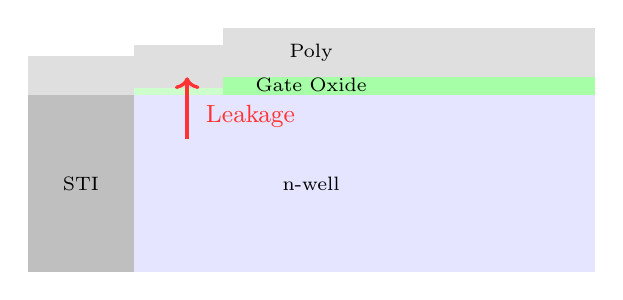
\begin{tikzpicture}[x=1.5cm,y=1.5cm, every node/.style={font=\scriptsize}]
  \begin{scope}[scale=1.5]
  \fill[blue!10,draw=none] (0,-1.0) rectangle (3.2,0);
  \node at (1.6,-0.5) {n-well};
  \fill[gray!50,draw=none] (0,-1.0) rectangle (0.6,0.0);
  \node at (0.3,-0.5) {STI};
  \fill[green!20,draw=none] (0.6,0.0) rectangle (1.1,0.04);
  \fill[green!35,draw=none] (1.1,0.0) rectangle (3.2,0.10);
  \node[black] at (1.6,0.06) {Gate Oxide};
  \fill[gray!25,draw=none] (0.0,0.0) rectangle (0.6,0.22);
  \fill[gray!25,draw=none] (0.6,0.04) rectangle (1.1,0.28);
  \fill[gray!25,draw=none] (1.1,0.10) rectangle (3.2,0.38);
  \node at (1.6,0.24) {Poly};
  \draw[->,very thick,red!80] (0.9,-0.25) -- (0.9,0.1);
  \node[red!80,anchor=west] at (0.95,-0.12) {\small Leakage};
  \end{scope}
\end{tikzpicture}
\caption{STI端部におけるゲート酸化膜シンニングとリーク経路}
\label{fig:sti_edge_leakage_gateoxide}
\end{figure}

解決策として、開発チームはLOCOSとSTIを組み合わせたハイブリッドプロセスを検討した。LOCOSの利点である高耐圧特性を保持しつつ、STIによる素子間隔縮小を導入することで歩留まり改善を狙ったのである。  
しかし、プロセスフローは複雑化し、工程数が大幅に増加した。結果として、当初の目標であった「50\%のコスト削減」は達成できず、むしろ工程コストの上昇が懸念される状況となった。

このハイブリッド統合の工程順序と設計上の要点を整理したのが**Fig.~\ref{fig:hybrid_flow}**である。  
LOCOSを先行してHV ブロックを形成し、その後にSTIプロセスでLVロジックを構築する。  
熱履歴の影響・素子分離構造のトレードオフ・BoAの効果を併せて最適化する必要がある。

\begin{figure*}[!t]
  \centering
  \resizebox{0.95\textwidth}{!}{%
  \begin{tikzpicture}[
    every node/.style={font=\footnotesize},
    node distance=9mm and 12mm,
    box/.style={draw, rounded corners, align=left, inner sep=4pt,
                minimum height=8mm, text width=0.46\textwidth, fill=gray!10},
    arrow/.style={-{Stealth}, thick},
    note/.style={align=left, text width=0.40\textwidth}
  ]

  % 左列(工程フロー)
  \node[box] (hv) {%
    \textbf{HV Block (30\,V) — LOCOS first}\\
    フィールド酸化/チャネルストップ/厚酸化膜\\
    長チャネル・オフセット構造
  };

  \node[box, below=of hv] (therm) {%
    \textbf{大熱履歴}\\
    高温酸化・ドライブインにより熱予算消費\\
    \emph{後続LV素子への影響に注意}
  };

  \node[box, below=of therm] (lv) {%
    \textbf{LV Logic (1.8\,V) — STI later}\\
    トレンチ形成→埋め込み酸化→CMP\\
    浅拡散・微細配線
  };

  \node[box, below=of lv] (finish) {%
    \textbf{後工程}\\
    メタル配線/パッシベーション/\textbf{BoAバンプ形成}
  };

  \draw[arrow] (hv) -- (therm);
  \draw[arrow] (therm) -- (lv);
  \draw[arrow] (lv) -- (finish);

  % 右列(注記)
  \node[note, right=14mm of therm] (risk) {%
    \textit{統合上のリスク}: LOCOSの高温熱履歴が\\
    1.8\,Vロジックの $V_{\mathrm{th}}$・リークに影響。\\
    $\Rightarrow$ 統合最適化(条件分離, マージン設計)が必要
  };
  \draw[arrow] (therm.east) -- (risk.west);

  \node[note, right=14mm of lv] (benefit) {%
    \textit{STIの効果}: 面積削減 $\Rightarrow$ ダイ縮小・コスト低減。\\
    \textit{BoAの効果}: パッド領域縮小がコストダウンの主役
  };
  \draw[arrow] (lv.east) -- (benefit.west);

  \end{tikzpicture}
  }% end resizebox
  \caption{LOCOS+STIハイブリッドのプロセス順序:HV(LOCOS)先行 $\rightarrow$ LV(STI) 後続。熱履歴の影響と面積削減のトレードオフ、BoAの寄与を併記。}
  \label{fig:hybrid_flow}
\end{figure*}

\section{BoA技術と評価方法}
CD50プロジェクトにおいて最も大きな成果の一つが、Bump on Active (BoA) 技術である。  
BoAは、従来パッド専用のデッドスペースに配置されていたバンプを、アクティブ領域上に直接形成する実装技術であり、パッド領域削減によるダイサイズの縮小を実現した。  
これはチップコスト削減に直結する革新的なアプローチであり、狭スクライブ技術と並んで、CD50における実質的なコストダウンの中核施策となった。

BoAの導入にあたっては、アクティブ素子上への荷重ストレスの影響を定量的に評価し、量産信頼性を確立することが必須であった。  
このため、開発チームは専用の大規模TEG (Test Element Group) を約3か月をかけて設計・作成し、広範囲の素子特性を体系的に評価した。  

\subsection{評価構成}
各素子について、以下の3つの条件を並列配置し、相互比較可能な形とした。
\begin{enumerate}
  \item 何も置かない素子(基準)
  \item AL Pad上の素子(従来方式)
  \item Bump Pad上の素子(BoA適用方式)
\end{enumerate}
この構成により、バンプ形成そのものが素子特性に与える影響を直接抽出できる設計とした。

% preamble に \usepackage{tikz} を読み込んでください

% preamble: \usepackage{tikz}
\begin{figure}[t]
\centering
\begin{tikzpicture}[scale=0.92, every node/.style={font=\footnotesize}]

% ===== 上:従来(外周Pad領域あり、片辺バンプ) =====
\node[align=center] at (3.2,6.15) {従来構造(外周Pad領域/片辺バンプ)};

% チップ外形(長辺Lは下図と同一)
\draw[thick] (0,5.0) rectangle (6.4,5.8);

% 外周Pad領域(薄色帯)
\fill[gray!20] (0,5.62) rectangle (6.4,5.80);
\node at (3.2,5.86) {\scriptsize Pad領域(従来のみ)};

% 片辺バンプ:Pad帯の中
\foreach \x in {0.5,1.3,2.1,2.9,3.7,4.5,5.3,6.1} {
  \draw[fill=black] (\x,5.71) circle (0.06);
}

% 長辺L(一定)
\draw[<->] (0,4.86) -- (6.4,4.86);
\node at (3.2,4.72) {長辺 $L$(一定)};

% 短辺 W_before
\draw[<->] (-0.35,5.00) -- (-0.35,5.80);
\node[rotate=90] at (-0.60,5.40) {$W_{\text{before}}$};


% ===== 下:BoA(Pad領域なし、片辺バンプを内側寄せ) =====
\node[align=center] at (3.2,3.95) {BoA構造(Pad領域なし/片辺バンプ)};

% チップ外形(上と完全同一の長辺L)
\draw[thick] (0,3.15) rectangle (6.4,3.75);

% 片辺バンプ:内側寄り(Active上を想定、帯は描かない)
\foreach \x in {0.5,1.3,2.1,2.9,3.7,4.5,5.3,6.1} {
  \draw[fill=black] (\x,3.68) circle (0.06);
}

% 長辺L(一定)
\draw[<->] (0,2.99) -- (6.4,2.99);
\node at (3.2,2.85) {長辺 $L$(一定)};

% 短辺 W_after
\draw[<->] (6.75,3.15) -- (6.75,3.75);
\node[rotate=90] at (7.00,3.45) {$W_{\text{after}}$};

% 短辺縮小と等価なPad幅(ΔW)を示す
\draw[decorate, decoration={brace, amplitude=5pt}] (6.40,5.80) -- (6.40,5.62);
\node[right] at (6.55,5.71) {\(\Delta W \approx W_{\text{pad}}\)};

% 短辺のみ縮小を強調
%\draw[->,thick] (6.75,5.40) -- (6.75,3.45) node[midway,right]{短辺のみ縮小};

\end{tikzpicture}
\caption{横長ドライバICの模式図。従来は外周Pad領域の上に\textbf{片辺バンプ}を並べるため短辺が大きい。
BoAではPad領域が不要となり、同じ片辺バンプを\textbf{内側寄せ}にできるため、\(\,W_{\text{before}}\to W_{\text{after}}\) へ短辺が縮小する。
長辺 \(L\) は両者で同一。}
\label{fig:boa_edge_bump_simple}
\end{figure}

\subsection{評価手順}
評価は以下の手順で行った。
\begin{enumerate}
  \item 初期ETESTにより素子の基本特性を測定
  \item バンプ荷重を加える(単発荷重および継続荷重の両方を実施)
  \item 荷重後にETESTを再測定し、特性変動やオープン/ショートの有無を確認
\end{enumerate}
特に、COF (Chip on Film) 実装を模擬した継続荷重評価では、実装後の長期信頼性を意識した検証を行った。

\begin{table}[htbp]
\centering
\caption{BoA評価におけるETEST対象素子}
\label{tab:etest_devices}
\begin{tabular}{|l|l|}
\hline
カテゴリ & 対象素子 \\
\hline
トランジスタ & LV MOS, HV MOS (特にHV PMOS) \\
キャパシタ   & MOSキャパシタ (ゲート酸化膜品質) \\
抵抗素子     & Active抵抗, Poly抵抗 \\
配線・接続   & 配線抵抗, ビア/コンタクトチェーン, 層間リーク \\
\hline
\end{tabular}
\end{table}

\begin{table}[htbp]
\centering
\caption{BoA荷重試験の区分と目的}
\label{tab:load_test}
\begin{tabular}{|l|l|l|}
\hline
評価種類 & 対象素子 & 評価目的 \\
\hline
一時荷重 & フルTEG & 素子破壊の有無を確認 \\
継続荷重 & 小規模TEG (MOS中心) & COF模擬下での長期信頼性評価 \\
\hline
\end{tabular}
\end{table}

\subsection{評価上の工夫}
通常ETESTはAL Pad経由で測定を行うが、今回のBoA評価ではBump Padを介して直接測定する必要があった。  
その結果、プローバ針先とバンプとの接触抵抗(10〜20~$\Omega$)が加算され、低抵抗素子測定において大きな測定ばらつきが生じた。  
これに対して、プローバの針先研磨プログラムを導入し、数回測定ごとに針先をリフレッシュすることで、接触抵抗の影響を最小化し、測定の再現性を確保した。

\begin{figure}[t]
  \centering
  \begin{tikzpicture}
    \begin{axis}[
      width=7cm, height=5cm,
      xlabel={測定回数},
      ylabel={抵抗値 [Ω]},
      ymin=0, ymax=30,
      grid=both,
      legend style={at={(0.5,-0.2)},anchor=north}
    ]
      \addplot+[mark=o] coordinates {
        (1,18)(2,20)(3,15)(4,25)(5,19)
      };
      \addlegendentry{研磨前}

      \addplot+[mark=triangle*] coordinates {
        (1,12)(2,11)(3,10)(4,12)(5,11)
      };
      \addlegendentry{研磨後}
    \end{axis}
  \end{tikzpicture}
  \caption{プローバ針先研磨による接触抵抗安定化効果}
\end{figure}

\subsection{意義}
これらの体系的評価により、BoAがアクティブ素子上であっても量産可能な信頼性を確保できることを実証した。  
さらに、荷重応力に対する素子特性の変動メカニズムを明らかにし、設計マニュアルに反映した点は、当時として先進的な取り組みであった。

\section{評価結果と課題}
BoA技術の信頼性検証として実施した一時荷重試験では、すべての素子において顕著な不具合や特性劣化は観測されなかった。  
この結果から、バンプ形成そのものや短期的な応力印加は、素子の動作に大きな悪影響を及ぼさないことが確認された。  

一方で、長期荷重試験(COF実装を模擬し、継続的に荷重を印加する試験)では、特にHV PMOSデバイスにおいて顕著な特性変動が観測された。  
具体的には、しきい値電圧やドレイン電流のシフトが確認され、その変動は荷重応力に起因するキャリア移動度の変化によるものと推定された。  
この結果は、PMOSが機械的応力に対してNMOSよりも感受性が高いという既知の物理的傾向と一致しており、評価結果の妥当性を裏付けるものであった。  

重要な点は、この変動値を定量的に整理し、設計マニュアルに反映したことである。  
これにより設計者は、実装応力を考慮したマージン設計を行うことが可能となり、量産における歩留まりと信頼性の確保に大きく貢献した。  
当時(2000年代前半)としては、機械的荷重による電気的特性変動を設計規則化した事例は少なく、非常に先進的な取り組みであったと言える。  

さらに、評価過程では測定技術上の課題も明らかになった。  
通常ETESTはAL Padを介して行うが、BoA評価ではBump Padを介して測定する必要があった。  
その結果、プローバ針先とバンプ間に10--20~$\Omega$の接触抵抗が付加され、特に配線抵抗などの低抵抗素子測定では測定値に大きなばらつきが生じた。  
この課題に対しては、プローバの針先研磨プログラムを導入し、一定回数ごとに針先をクリーニングすることで接触抵抗をリセットし、測定の安定性を確保する手法を確立した。  

このように、BoA評価は単なる素子信頼性の確認に留まらず、計測インフラや設計規則の整備を伴う包括的な技術確立プロセスであった。

\section{なぜHV PMOSが影響を受けやすいか}
HV PMOSデバイスにおける特性変動の顕著さには、いくつかの物理的要因が関与している。  

まず、HV PMOSは厚いゲート酸化膜と長いチャネル長を特徴とする構造を有しており、この構造は応力集中を引き起こしやすい。  
特に、LDD(Lightly Doped Drain)領域やオフセット構造における機械的応力の集中は、キャリア輸送特性の変動を増幅する要因となる。  

次に、PMOSデバイスにおけるホール移動度は、NMOSにおける電子移動度に比べて結晶歪みや応力の影響を強く受けやすい。  
圧縮応力や引張応力の持続印加によってバンド構造や界面準位状態が変化し、しきい値電圧や移動度の変動として現れやすい。  

さらに、長期荷重下では一時的な弾性的変形だけでなく、界面準位の増加や応力緩和過程が進行し、時間依存的な特性劣化として顕在化する。  
このため、一時荷重試験では問題が生じなかったにもかかわらず、継続荷重試験においてHV PMOSでのみ変動が顕著となった。  

以上のことから、HV PMOSは応力感受性の高い素子として実装時に特に注意が必要であり、設計段階でのマージン設定やパッケージ・実装設計との協調が不可欠であることが明らかとなった。

\section{結果と影響}
BoA技術は、技術的には量産化に成功し、従来プロセスに比べて大幅なダイサイズ削減を実現した。  
特に、狭スクライブとの併用により、理論的にはチップ面積当たりのコスト競争力を大幅に改善できることが示された。  
この成果は、CD50プロジェクトにおける数少ない実質的なコストダウン施策として評価された。

しかし、国際市場での競争環境においては、BoAの成功だけでは十分ではなかった。  
Samsungは大規模投資と量産能力を背景に、極めて低価格なチップを提示し、価格競争の主導権を握った。  
結果として、エプソンが当初優位性を持っていた
\begin{itemize}
  \item 0.35 µm モノクロドライバ
  \item 0.25 µm カラードライバ
\end{itemize}
といった主要製品群においてもシェアを急速に失い、競合の台頭を止めることはできなかった。

さらに、BoAのような実装技術革新があったにもかかわらず、プロセス微細化の流れにおいては0.13 µm以降への移行に成功できず、国際標準から取り残される結果となった。  
微細化の停滞はチップ性能やコスト面での差を一層拡大させ、最終的に事業としての継続を困難にした。

この事例は、技術的ブレークスルーがあっても、市場競争における価格戦略や量産スケールの差を覆すことは難しいことを示している。  
エプソンの半導体事業部にとってBoAは「最後の攻防」とも言える挑戦であったが、Samsungの台頭と国際的微細化トレンドに押され、産業競争力の低下を防ぐには至らなかった。

結果的に、エプソンは業界におけるリーダーシップを喪失し、日本の半導体メーカー全体が直面した「技術は成功しても事業として敗北する」という歴史的パターンの一例となった。

\section{結論}
CD50プロジェクトは、当初の目的であった「50\%のコスト削減」を直接的に達成することはできなかった。  
0.18 µm STIによるHVデバイス集積は技術的課題により断念され、LOCOS+STIハイブリッドプロセスへの移行はコスト増を招いた。  
しかしその一方で、Bump on Active (BoA) 技術は量産化に成功し、ダイサイズ削減という形で明確な成果を残した。  
この点においてCD50は「部分的技術成功」と評価できる。

一方で、国際市場の現実はBoAの成功を超える厳しさを持っていた。  
Samsungを筆頭とする海外メーカーは、巨額投資と量産スケールを背景に圧倒的な価格競争力を示し、エプソンは優位を誇った0.35 µmモノクロドライバや0.25 µmカラードライバの領域でもシェアを喪失した。  
さらに0.13 µm以降の微細化に対応できなかったことが致命的となり、事業継続は困難となった。

この事例は、日本の半導体産業が直面した本質的な課題を象徴している。  
すなわち、\textbf{「技術的成功が必ずしも事業的成功には直結しない」} という乖離である。  
優れた技術革新があっても、国際競争においてはコスト、スケール、価格戦略といった要素が支配的であり、技術単独では市場の主導権を維持できない。  

産業史的観点から見ると、CD50プロジェクトは日本半導体産業全体の縮図であり、1990年代以降に進行した「日の丸半導体」の衰退過程を象徴的に示している。  
今後の技術開発においては、技術革新を事業戦略や国際競争力といかに結びつけるかが重要であり、本事例はその教訓を示す歴史的ケーススタディと位置付けられる。

\section*{謝辞}
本研究の一部は、エプソン半導体事業部における技術開発活動の成果に基づいている。  
特に、CD50プロジェクトおよびBoA技術の立ち上げに携わった設計・プロセス・実装・評価の各チームの尽力なしには、本稿で示した知見は得られなかった。  
当時の現場技術者・研究者の創意工夫と継続的努力に深く感謝する。  

また、本研究の背景には、液晶ディスプレイ市場の急速な拡大と、それに伴う国際的な価格競争の激化があった。  
Samsungをはじめとする海外メーカーとの厳しい競争環境は、エプソンの開発活動に大きな緊張感と革新をもたらし、その圧力がBoAのような先進技術を生み出す原動力となったことも記しておきたい。  

最後に、本稿の執筆にあたり、当時の経験や技術成果を整理し、半導体産業史的な観点から再評価する機会を与えてくれた同僚研究者や関係者各位に謝意を表する。

\begin{thebibliography}{99}

\bibitem{Sze2006}
S. M. Sze and K. K. Ng, \textit{Physics of Semiconductor Devices}, 3rd ed. Hoboken, NJ, USA: Wiley-Interscience, 2006.

\bibitem{Colinge2004}
J.-P. Colinge, \textit{Silicon-On-Insulator Technology: Materials to VLSI}, 3rd ed. Boston, MA, USA: Springer, 2004.

\bibitem{ITRS2001}
International Technology Roadmap for Semiconductors (ITRS), 2001 Edition. [Online]. Available: \url{http://www.itrs2.net}

\bibitem{Yamada1999}
H. Yamada, T. Suzuki, and M. Takahashi, ``High-voltage CMOS devices using shallow trench isolation (STI) for display driver applications,'' in \textit{Proc. IEEE Int. Symp. Power Semiconductor Devices and ICs}, 1999, pp. 237--240.

\bibitem{Park2003}
J. Park, H. Kim, and S. Lee, ``Cost-effective driver IC technologies for TFT-LCD panels,'' in \textit{SID Symp. Digest Tech. Papers}, vol. 34, no. 1, 2003, pp. 456--459.

\bibitem{Oshima2008}
K. Oshima, ``The rise and fall of the Japanese semiconductor industry,'' \textit{IEEE Micro}, vol. 28, no. 2, pp. 74--83, Mar./Apr. 2008.

\bibitem{Samizo2025}
S. Samizo, ``CD50 project and bump on active (BoA) case study: The last struggle of Epson semiconductor division,'' unpublished manuscript, 2025.

\end{thebibliography}

\section*{著者略歴}
\textbf{三溝 真一 (Shinichi Samizo)} は、信州大学大学院 工学系研究科 電気電子工学専攻にて修士号を取得した。  
その後、セイコーエプソン株式会社に勤務し、半導体ロジック/メモリ/高耐圧インテグレーション、さらにインクジェット薄膜ピエゾアクチュエータおよび PrecisionCore プリントヘッドの製品化に従事した。  
現在は独立系半導体研究者として、プロセス/デバイス教育、メモリアーキテクチャ、AIシステム統合などの研究に取り組んでいる。  
連絡先: \href{mailto:shin3t72@gmail.com}{shin3t72@gmail.com}

\end{document}
